\usepackage[inner=3cm, outer=2.2cm, top=2.7cm, bottom=3cm,
            headheight=16pt]{geometry}

%\usepackage[Bjarne]{fncychap}

\usepackage[pages=some]{background}
\backgroundsetup{
scale=1,
color=black,
opacity=0.1,
angle=0,
contents={%
  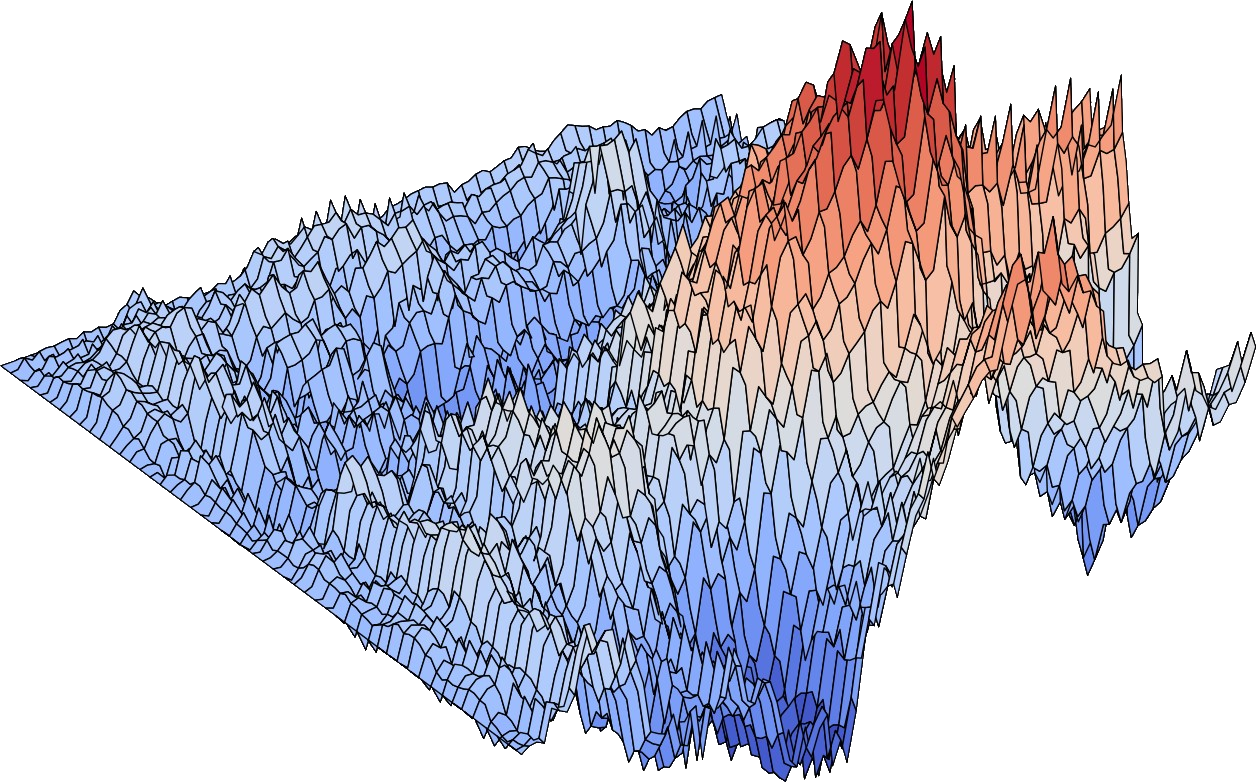
\includegraphics[height=0.6\paperheight]{browniansheet.png}
  }%
}
\usepackage{emptypage}
\usepackage{fancyhdr}
\pagestyle{fancy}
\renewcommand{\chaptermark}[1]%
{\markboth{\thechapter.\ \textsc{#1}}{}}
\renewcommand{\sectionmark}[1]%
{\markright{\thesection.\ #1}}
\fancyhf{}
\fancyhead[LE,RO]{\thepage}
\fancyhead[CO]{\rightmark}
\fancyhead[CE]{\leftmark}
%\renewcommand{\footrulewidth}{0.4pt}
%\fancyfoot[LE]{}
%\fancyfoot[RO]{\thedate}

\fancypagestyle{plain}{%
  \fancyhf{} % remove everything
  \renewcommand{\headrulewidth}{0pt} % remove lines as well
  \renewcommand{\footrulewidth}{0pt}
  \fancyfoot[C]{\thepage}
}

\def\thelecture{}%
\newcommand{\lecture}[3]{
    \def\thelecture{#3}
%    \chapter{\thelecture}
}

% Pour obtenir une numérotation des équations de la forme
% Chapitre.Section.Numéro
\usepackage{chngcntr}
\counterwithin{equation}{section}